% !TEX root = ../zz-lecture.tex


\chapter{角动量及其守恒}

研究质点的运动时,经常用动量$ \vec{p}=m\vec{v} $描述质点的运动状态,它包含了质点运动速度的大小和方向特征。
但是当质点(或质点系)绕某一固定点(或轴线)运动时,不仅质点的动量时刻改变,质点离固定点的距离和方位也在改变,这时很难用动量完整地揭示其规律,我们可以尝试引入新的物理量来更方便的描述这类运动。
例如,当行星绕太阳公转时,行星的轨迹是以太阳为焦点的一个椭圆,如图所示。
行星在不同位置的速度大小和方向都不同。
由开普勒第二定律可知,行星与太阳连线在相等时间内扫过的面积相等,在A、B、C位置分别取$ \Delta t\rightarrow 0 $的相等时间$ \Delta t $,
\[
r_1 (v_1 \Delta t)sin\frac{\pi}{2} = r(v\Delta t)\sin\alpha = \text{const.}
\]
即
\[
rv\sin\alpha = \const
\]
考虑到不同行星质量不同,因此对任一行星用它的质量与上式相乘以后得到的$r(mv)sin⁡\alpha = \const$这表明$r(mv)sin\alpha⁡$也是反映物体运动属性的物理量,我们把这个物理量叫做角动量,也叫动量矩。


\begin{example}
	%%%%题干
	如图所示,质量为$ m $的小球自由下落,某时刻具有速度$ v $,此时小球与图中的A、B、C三点恰好位于某长方形的四个顶点,且小球与A,C两点的距离分别为$ l_1 $、$ l_2 $,求小球相对A、B、C三点的角动量$ L_1 $、$ L_2 $、$ L_3 $的大小.
	%%%%插图
		\marginpar{\centering 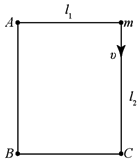
\includegraphics[width=0.6\marginparwidth]{image/am-2.png}\figcaption{第\theexample 题 } }
	
	\begin{taggedblock}{student}
		\vspace*{2cm}
	\end{taggedblock}
	
	
	%%%%答案
	\begin{taggedblock}{answer}
		答案:$ L_1 = mvl_1,L_2 = mvl_1,L_3=0 $
	\end{taggedblock}
	
	
	%%%%解析
	\begin{taggedblock}{analysis}
		解析:
	\end{taggedblock}
\end{example}


\begin{example}
	%%%%题干
	 质量为M的质点固定不动,在万有引力作用下,质量为$ m $的质点绕着它做半径为R的圆周运动.取圆轨道上的P点为参考点,如图所示,试求:
	 
	 ( 1 )在图中点1处,m相对P点的角动量大小$ L_1 $.
	 
	 ( 2 )在图中点2处,m相对P点的角动量大小$ L_2 $.
	 
	%%%%插图
		\marginpar{\centering 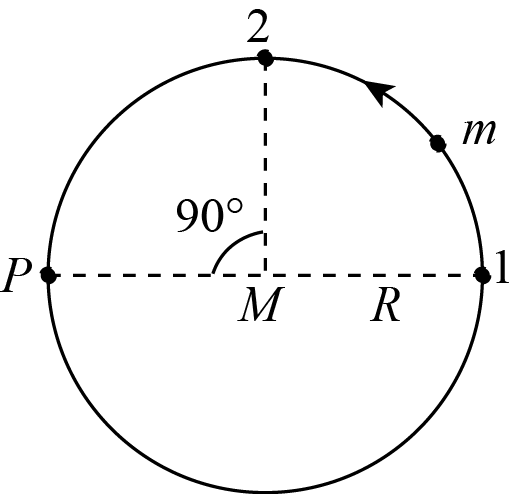
\includegraphics[width=0.8\marginparwidth]{image/am-3.png}\figcaption{第\theexample 题 } }
	
	\begin{taggedblock}{student}
		\vspace*{1cm}
	\end{taggedblock}
	
	
	%%%%答案
	\begin{taggedblock}{answer}
		答案:$ L_1 = 2m\sqrt{GMR,L_2 = m\sqrt{GMR}} $
	\end{taggedblock}
	
	
	%%%%解析
	\begin{taggedblock}{analysis}
		解析:
	\end{taggedblock}
\end{example}


\begin{example}
	%%%%题干
	在光滑的水平面上,两个质量分别为$ m_1 $和$ m_2 $的小球,用长为$ l $的轻线连结.开始时,线正好拉直,$ m_1 $和$ m_2 $的速度分别为$ v_1 $和$ v_2 $(v$v_1>v_2) $,它们的方向相同,且垂直于连线,求系统相对质心的总角动量为多大.
	%%%%插图
	%	\marginpar{\centering \includegraphics[width=0.8\marginparwidth]{image/}\figcaption{第\theexample 题 } }
	
	\begin{taggedblock}{student}
		\vspace*{1cm}
	\end{taggedblock}
	
	
	%%%%答案
	\begin{taggedblock}{answer}
		答案:$ \frac{m_1m_2}{m_1+m_2}(v_1-v_2)l $
	\end{taggedblock}
	
	
	%%%%解析
	\begin{taggedblock}{analysis}
		解析:根据定义直接计算。
	\end{taggedblock}
\end{example}


下面我们不加证明地给出角 动量守恒定律。
当物体相对某一固定点的合外力矩等于零时,物体相对这一点的角动量保持不变,此即角动量守恒定律。
注意:角动量守恒定律不仅可以对质点应用,也可以对质点组应用,这时只要求合外力矩为零,不需要考虑内力力矩。当质点组对固定点的合外力矩为零时,质点组对固定点的总角动量守恒。
当所选参考系不是惯性系时,要考虑非惯性力的力矩,当然我们一般不涉及这些复杂情况。
具体来说,角动量守恒的成立条件有以下情况:

\begin{itemize}
	\item 物体不受外力;
	
	\item 物体所受外力均通过固定点,故各力相对该点的力矩均为零
	
	\item 物体所受各个外力的力矩不为零,但外力矩的矢量和为零
\end{itemize}

回到上面的行星绕太阳运动的例子,行星所受万有引力通过太阳,故行星所受外力相对于太阳的合外力矩为零,因此,行星的角动量守恒。开普勒第二定律本质上反映的正是角动量守恒定律。

\begin{example}
	%%%%题干
	如图所示,对于圆锥摆,摆球相对于运动中心$ O_1 $的角动量是否守恒.
	%%%%插图
	%	\marginpar{\centering 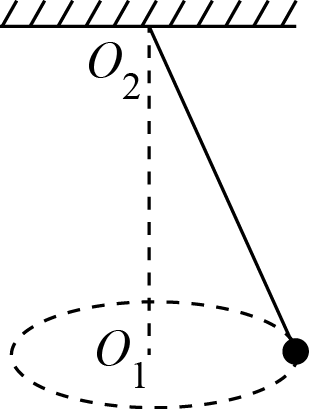
\includegraphics[width=0.8\marginparwidth]{image/am-4.png}\figcaption{第\theexample 题 } }
	
	\begin{taggedblock}{student}
		\vspace*{1cm}
	\end{taggedblock}
	
	
	%%%%答案
	\begin{taggedblock}{answer}
		答案:守恒
	\end{taggedblock}
	
	
	%%%%解析
	\begin{taggedblock}{analysis}
		解析:摆球所受重力和拉力的合力为圆周运动的向心力,刚好指向$ O_1 $,故合外力矩为零,角动量守恒.
	\end{taggedblock}
\end{example}


\begin{example}
	%%%%题干
	如图所示,一个质量为$ m $的小球系于一根不能伸长的轻绳一端,放在光滑水平桌面上,绳的另一端穿过桌面上的小孔用手拉住,先给小球一个大小为$ v_1 $的速度,使它沿半径为$ r_1 $的圆轨道运动,然后慢慢向下拉绳,使小球的转动半径减小至$ r_2 $,试求这时小球的速率.
	%%%%插图
	%	\marginpar{\centering \includegraphics[width=0.8\marginparwidth]{image/}\figcaption{第\theexample 题 } }
	
	\begin{taggedblock}{student}
		\vspace*{2cm}
	\end{taggedblock}
	
	
	%%%%答案
	\begin{taggedblock}{answer}
		答案:$ v_2 = \frac{r_1}{r_2}v_1 $
	\end{taggedblock}
	
	
	%%%%解析
	\begin{taggedblock}{analysis}
		解析:小球对O点的合外力矩为零,因此小球对O点的角动量守恒,即$ mv_1 r_1=mv_2 r_2 $,解得$ :v_2=r_1/r_2  v_1 $.
	\end{taggedblock}
\end{example}

\begin{example}
	%%%%题干
	 光滑水平面上有一小球A被一轻绳拴住,轻绳穿过平面上小孔O与小球B连接.开始时A球在水平面上绕O做匀速圆周运动,B球静止地向下垂挂着,如图所示.今使小球B的质量缓慢增加,直到A球绕O点做圆周运动的半径缩小一半,试问此时B球质量为初始质量的多少倍.
	%%%%插图
		\marginpar{\centering 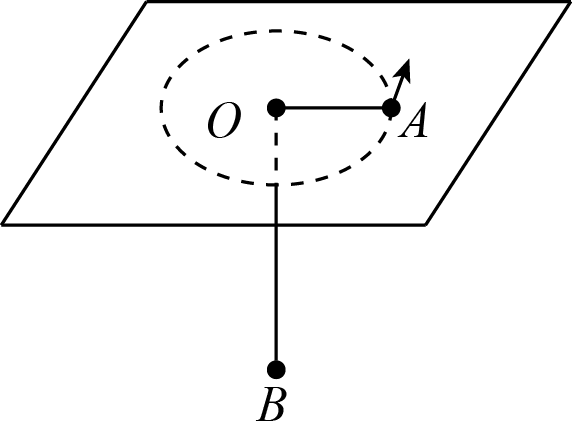
\includegraphics[width=0.8\marginparwidth]{image/am-5.png}\figcaption{第\theexample 题 } }
	
	\begin{taggedblock}{student}
		\vspace*{2cm}
	\end{taggedblock}
	
	
	%%%%答案
	\begin{taggedblock}{answer}
		答案:8
	\end{taggedblock}
	
	
	%%%%解析
	\begin{taggedblock}{analysis}
	\begin{center}
		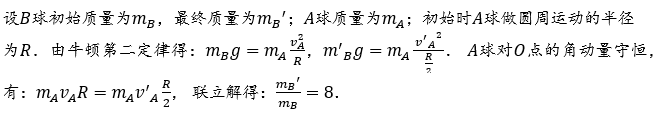
\includegraphics[width=0.9\linewidth]{image/am-6}
	\end{center}
	
	\end{taggedblock}
\end{example}


\begin{example}
	%%%%题干
	如图所示,在水平的光滑桌面上开有一个小孔,条绳穿过小孔,其两端各系由一质量为$ m $的物体,开始时,用手握住下面的物体,桌上的物以$ v_0 = \frac{3}{2}\sqrt{2gr_0} $速率作半径为$ r_0  $(即桌上部分绳长)的匀速圆周运动,然后放手,求以后运动中桌上绳索的最大长度.
	%%%%插图
	%	\marginpar{\centering 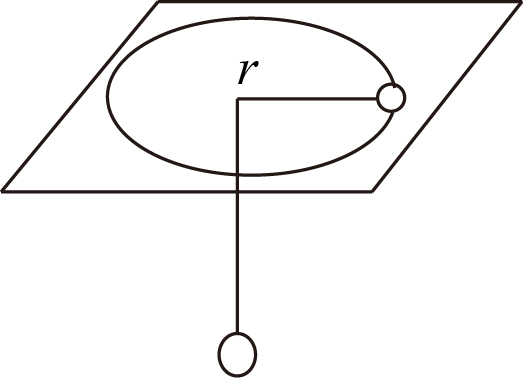
\includegraphics[width=0.8\marginparwidth]{image/am-7.png}\figcaption{第\theexample 题 } }
	
	\begin{taggedblock}{student}
		\vspace*{2cm}
	\end{taggedblock}
	
	
	%%%%答案
	\begin{taggedblock}{answer}
		答案:$ r_1 = 3r_0 $
	\end{taggedblock}
	
	
	%%%%解析
	\begin{taggedblock}{analysis}
		\begin{center}
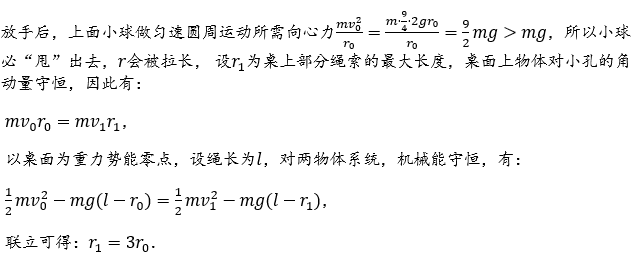
\includegraphics[width=0.9\linewidth]{image/am-8}
\end{center}

	\end{taggedblock}
\end{example}


\begin{example}
	%%%%题干
	 如图所示,a为一固定放置的半径为$ R $的均匀带电球体,O为球心.已知取无限远处的电势为零时,球表面处的电势为$ U = 1000~\si{V} $.在离球心O很远的O'点附近有一质子,它以$ E_k = 2000~\si{eV} $的动能沿与OO'平行的方向射向a.
	 以$ l $表示质子与OO'线之间的垂直距离,要使质子能够与带电球体a的表面相碰,试求$ l $的最大值.
	%%%%插图
	%	\marginpar{\centering \includegraphics[width=0.8\marginparwidth]{image/}\figcaption{第\theexample 题 } }
	\begin{center}
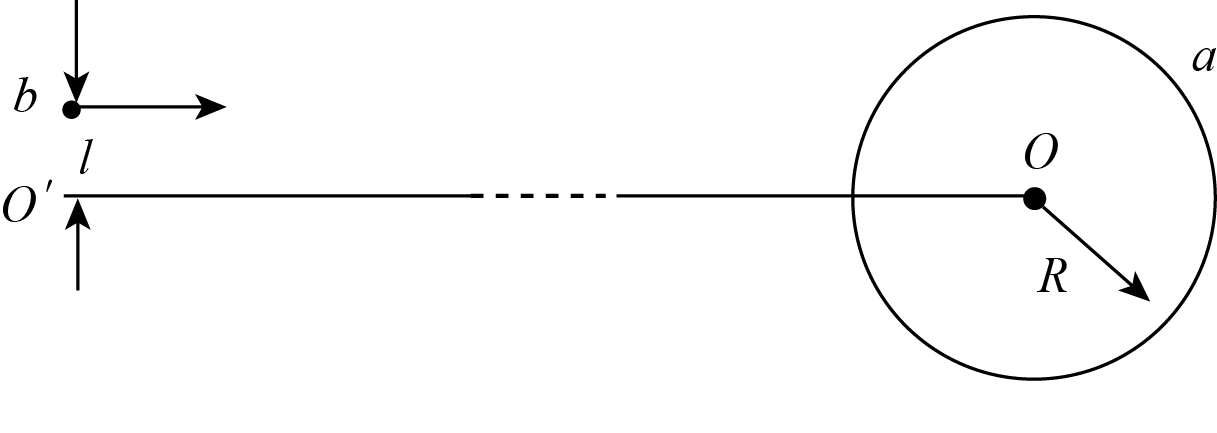
\includegraphics[width=0.4\linewidth]{image/am-9}
\end{center}

	\begin{taggedblock}{student}
		\vspace*{2cm}
	\end{taggedblock}
	
	
	%%%%答案
	\begin{taggedblock}{answer}
		答案:$ \frac{\sqrt{2}}{2}R $.
	\end{taggedblock}
	
	
	%%%%解析
	\begin{taggedblock}{analysis}
\begin{center}
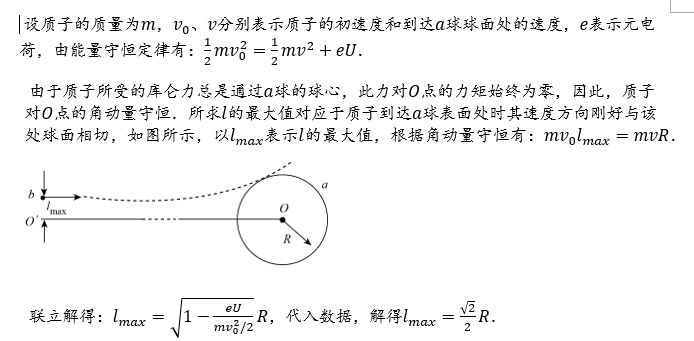
\includegraphics[width=0.9\linewidth]{image/am-10}
\end{center}

	\end{taggedblock}
\end{example}


\begin{example}
	%%%%题干
	如图所示,两个同样重的小孩,各抓着跨过滑轮绳子的两端.一个孩子用力向上爬,另一个小孩则抓住绳子不动.若滑轮的质量和轴上的摩擦都可忽略,不计绳子质量,哪个小孩先到达滑轮.
	%%%%插图
		\marginpar{\centering 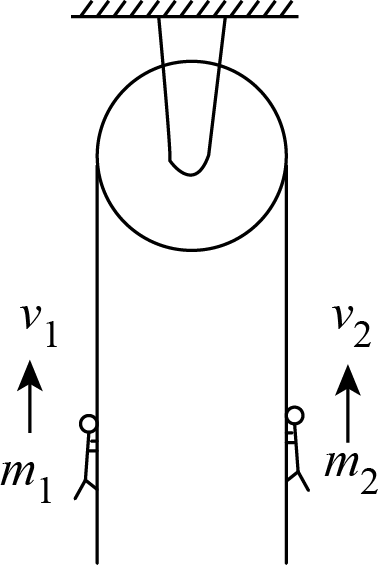
\includegraphics[width=0.8\marginparwidth]{image/am-11.png}\figcaption{第\theexample 题 } }
	
	\begin{taggedblock}{student}
		\vspace*{2cm}
	\end{taggedblock}
	
	
	%%%%答案
	\begin{taggedblock}{answer}
		答案:同时到达滑轮
	\end{taggedblock}
	
	
	%%%%解析
	\begin{taggedblock}{analysis}
		解析: 设两个小孩的质量为$ m $,向上的速度分别为$ v_1 $、$v_2$,滑轮的半径为$R$.由于两个小孩对轴的重力矩大小相等、方向相反,因此两个小孩组成的系统对转轴的角动量守恒,有:$mv_1 R=mv_2 R$,解得:$v_1=v_2$,因此他们同时到达滑轮.
	\end{taggedblock}
\end{example}


\begin{example}
	%%%%题干
	轻杆可以围绕固定点O自由无阻力转动,质量为$ 2m $的A球开始固定在轻杆的中点,质量为$ m $的B球固定在杆的下方端点处,一个质量也为m的球C以速度$ v $入射,并且入射后与B粘连在一起,求碰后B的速度多大.
	%%%%插图
		\marginpar{\centering 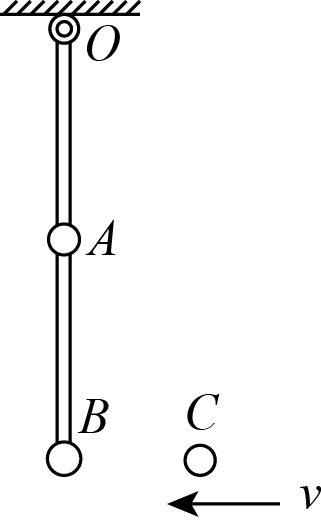
\includegraphics[width=0.6\marginparwidth]{image/am-12.png}\figcaption{第\theexample 题 } }
	
	\begin{taggedblock}{student}
		\vspace*{2cm}
	\end{taggedblock}
	
	
	%%%%答案
	\begin{taggedblock}{answer}
		答案:$ \frac{2}{5}v $
	\end{taggedblock}
	
	
	%%%%解析
	\begin{taggedblock}{analysis}
		\begin{center}
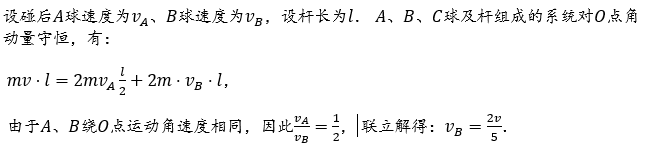
\includegraphics[width=0.9\linewidth]{image/am-13}
\end{center}

	\end{taggedblock}
\end{example}


\begin{example}
	%%%%题干
	如图所示,一根质量可以忽略的细杆,长为$ 2l $,两端和中心处分别固连着质量为$ m $的小球B、D和C,开始时静止在光滑的水平桌面上.桌面上另有一质量为$ M $的小球A,以一给定速度$ v_0 $沿垂直于杆DB的方向与右端小球B作弹性碰撞.求刚碰后小球A、B、C、D的速度.
	%%%%插图
		\marginpar{\centering 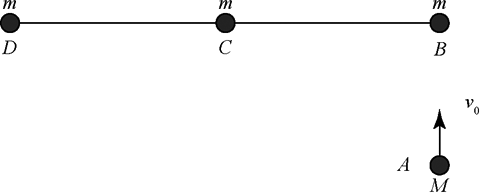
\includegraphics[width=\marginparwidth]{image/am-14.png}\figcaption{第\theexample 题 } }
	
	\begin{taggedblock}{student}
		\vspace*{2cm}
	\end{taggedblock}
	
	
	%%%%答案
	\begin{taggedblock}{answer}
		答案:
	\end{taggedblock}
	
	
	%%%%解析
	\begin{taggedblock}{analysis}
		\begin{center}
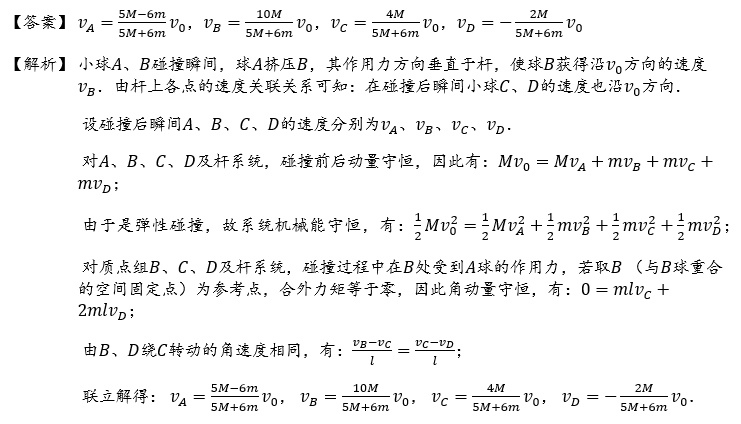
\includegraphics[width=0.9\linewidth]{image/am-15}
\end{center}

	\end{taggedblock}
\end{example}


\begin{example}
	%%%%题干
	如图所示,给静止在水平粗糙地面上的木块一初速度,使之开始运动.一学生利用角动量来考查此木块以后的运动过程:“把参考点设于如图所示的地面上一点O,此时摩擦力∫的力矩为零,从而地面上木块的角动量将守恒,这样木块将不减速而做匀速运动”.请指出上述推理的错误,并给出正确的解释.
	%%%%插图
		\marginpar{\centering 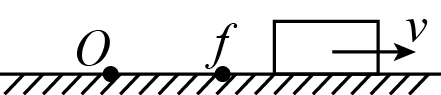
\includegraphics[width=\marginparwidth]{image/am-16.png}\figcaption{第\theexample 题 } }
	
	\begin{taggedblock}{student}
		\vspace*{1cm}
	\end{taggedblock}
	
	
	%%%%答案
	\begin{taggedblock}{answer}
		答案:
	\end{taggedblock}
	
	
	%%%%解析
	\begin{taggedblock}{analysis}
		解析:该学生未考虑竖直方向木块所受的支持力和重力的力矩.由于木块不发生偏转,故支持力的作用线不可能在质心上,否则绕质心的合力矩不可能为零.实际上支持力的作用线在重力作用线的右侧,支持力与重力的合力矩不为零,木块的角动量不守恒,与木块做减速运动不矛盾.
		故答案为:该学生未考虑竖直方向木块所受的支持力和重力的力矩.由于木块不发生偏转,故支持力的作用线不可能在质心上,否则绕质心的合力矩不可能为零.实际上支持力的作用线在重力作用线的右侧,支持力与重力的合力矩不为零,木块的角动量不守恒,与木块做减速运动不矛盾.
		
	\end{taggedblock}
\end{example}